\chapter[Introduction]{Introduction}
\label{ch:motivation}

\chapterepigraph{If you aren't sure which way to do something, then do it both ways and see which works better.}{John Carmack}

\newthought{Functional programming} (FP) has a long history, with its roots in the $\lambda$-calculus of Alonzo Church.\citefix[-1.5em]{church1932} One of the first functional programming languages was Lisp, invented by John McCarthy in 1958, which is still used today, over 50 years later.\citepage{reilly2003}{pages 156--157} Various languages have refined and extended the functional paradigm over the years --- probably the most notable as of now being Haskell, Scala, OCaml, F\#, and Erlang.

Despite the amount of time such languages have been available, use in industry has typically been far less than that of languages such as C, C++, and Java.\citepage[-2em]{odersky2010programming}{page 11} That being said, in recent years there has been increasing use of functional techniques and languages in certain areas. Erlang was designed for the development of highly fault tolerant telecommunication systems.\cite[-1em]{armstrong2007history} OCaml is used extensively by some organisations in the financial sector to create trading algorithms and other similar applications.\citefix[1em]{minsky2011ocaml} Scala is also increasingly popular, helped in part by its compatibility with the Java Virtual Machine (JVM) and object oriented design.

One of the often cited reasons against the use of functional programming in some domains is that of performance. This is due in part to mutable data structures generally being easier to represent on machine hardware; and it therefore being harder for functional compilers to convert the code into an efficient representation.\citefix{paulson1996ml} However, it is not a given that any program would run slower if written in a functional language: in some cases lazy-evaluation or compiler optimisations made possible by immutability can mean a program runs faster, plus advanced compiler techniques such as array fusion can lead to programs nearing the efficiency of hand-crafted C. And with modern machines getting ever faster, the domain of problems that require high levels of efficiency is getting smaller.

Performance problems alone cannot account for the fringe position of functional programming. The efficacy of the functional approach has been touted for many years,\sidenote{For example see \bibentry{hughes1989functional}.} yet it is still rare for mainstream projects to make any use of functional languages.

Instead of researching and discussing the theoretical advantages of the functional paradigm, this project will attempt to demonstrate the value of functional programming by utilising it in a problem domain that should pose a significant challenge that is not normally considered a `good' domain for FP. The chosen application for the project is a game.

\section{Why a Game?}

Game programming brings together a diverse range of computing areas. For example human interaction in real time, detailed graphics and animation, artificial intelligence / planning, networking, and various other dynamic elements.\sidenote{See \bibentry{crawford1984art}.} A game is also a tangible, sizeable piece of software, yet achievable for a four person group over two terms.

As well as demonstrating FP over a wide range of areas, a game also represents a serious business venture.\cite{essentialFacts2012} Computer games have been a huge industry for almost as long as personal computers have existed. Demand is high, and a vast amount of games are being continually developed, from triple-A ventures and big companies, down to indie companies and fan groups.

This project will certainly not be the first game ever to be developed in a functional language, nor is it likely to be the last. The project shall therefore not only deliver the finished game, but fully document the process --- explaining what went well and how the functional approach benefited the construction, as well as what proved challenging.

\section{Picking the Language}

There are several functional languages that would be suitable for this project, most of which have already been mentioned. Of these, the language chosen is Haskell. The reasons for this are outlined below.

\begin{description}
	\item[Concision] Haskell code is concise, yet readable. This is a very real advantage as it allows both for fast writing of code, as well as fast refactoring and maintenance. 
	\item[Purity] Haskell is a pure functional language, with all the advantages that gives. However side-effects and mutability are needed for real programs (especially games) and Haskell has excellent tools for solving these problems, via the IO Monad, State monads, etc. The `do' syntactic sugar makes Haskell one of the best languages for this.
	\item[Speed] Haskell has very good compiler support, and the Glasgow Haskell Compiler (GHC) is capable of producing highly efficient code. 
	\item[Type System] Haskell has a very advanced type system, which makes bugs and errors in refactoring easy to detect quickly. Automatic type inference allows for these advantages without the type system slowing down the programmer.
	\item[Testing] The purity of Haskell enables automated testing techniques not possible even in other functional languages. There are also well supported testing libraries available for both pure and impure code.
	\item[Community and Library Support] The Haskell community is very active and there are extensive libraries available for it. Due to Haskell compiling to C, most C system libraries have Haskell bindings. There are OpenGL and OpenAL, for example.
	\item[Familiarity] All members of the group have some experience with Haskell, and consider developing with it to be very enjoyable.
\end{description}

\section{Existing Systems}

To avoid confusion we shall consider separately research into functional programming for games, and what game we will actually make given current and historic trends in gaming.

\subsection{Existing research into Functional Programming of Games}

One of the most well known games written in a functional language (Haskell, as it happens) is \emph{Raincat}\sidenote{Source available online from \url{raincat.bysusanlin.com}.} written in Haskell and developed by Carnegie Mellon students in 2008. There is also a game company, \emph{ipwn studios}, who exclusively use Haskell for their products.\sidenote{See their website: \url{ipwnstudios.com}.} Despite this, there is little work on the academic research side that supports or opposes functional languages for games. 

There was a similar project in 2005 by Mun Hon Cheong, an undergraduate at the University of New South Wales;\cite{cheong2005functional} and though Cheong did manage to create a complete 3D game and gave detailed descriptions of some of the code techniques, the project did not provide a detailed insight into what exactly was effective, or challenging, about the use of a functional language.

The fact that an exhaustive search of the literature in this area revealed only a single undergraduate dissertation highlights the paucity of available research in this area, and coupled with the growing interest in functional languages for game development shows the case for this project.

\subsection{Existing Games}

Needless to say, the complete history of gaming, even if only restricted to computer games, would be too lengthy to examine here. The gaming industry has grown hugely since the early commercial computer game systems, in parallel with the huge developments in the capabilities of computers themselves. And while some games today are magnificent technical achievements with breathtakingly detailed graphics, sounds, and physics engines, there are many popular titles from indie game companies using only 2D graphics and simple engines enjoying success. It is not just the cutting edge of technology that can make a game fun.\sidenote{This is a complex issue. For a more complete treatment see \bibentry{malone1981makes}.}

In order to serve the purposes of the project, it will be necessary to create a game designed to compete in the current market. This doesn't mean it has to be as complete, complex, or technically sophisticated as a triple-A title, but it does have to be a game that, if fleshed out fully, would be considered fun and suitable for a small company or similar organisation to sell. Without this any conclusions drawn about the efficacy of the approach will not be sufficiently valid to developers.

For this reason it is worth briefly reviewing a few games --- some modern, some less so --- in order to identify what would be an appropriate brief for a game to help achieve the project's aims.

\begin{marginfigure}
	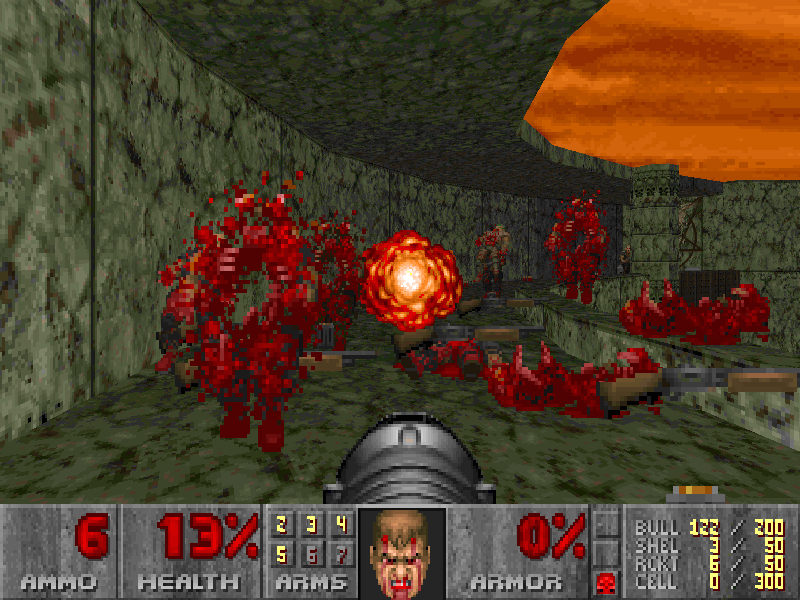
\includegraphics[width=6cm]{res/doom/doom.png}
	\caption{A screen from \emph{Ultimate Doom} (1995)}
	\label{fig:doom}
\end{marginfigure}

An early game that was hugely successful, as well as controversial, is \emph{Doom}, a first person shooter developed by John Carmack and John Romero of id Software and released in 1993. Doom was marketed using a shareware model --- the first third of the game being distributed for free, and the rest available for purchase. Doom represented a revolution in what was possible in a computer game, and is widely accepted as the game that popularised the first-person genre. The slickness of the graphics engine, the thought provoking levels and puzzles, the controversial satanic imagery, all contributed to Doom's success. But arguably the greatest innovation with the most effect on future gameplay was its multiplayer modes. Over modem or local serial connections, players could join forces to complete the main game, but could also battle each other in violent showdowns, coined \emph{deathmatches} by Romero. The name stuck.

Even though Doom is now very old, and the graphics look hugely out of date, it is still relevant to consider just how successful the multiplayer model in Doom was and still is. Battles are short, skilful, and highly addictive. Carmack and Romero predicted that Doom would become the number one cause of non-work in offices across the world, and they were right. Especially given the limited time constraints of the project, and the amount of writing time single player plot lines can involve, a compelling multiplayer mechanic would be a sound basis for the new game.

\begin{marginfigure}
	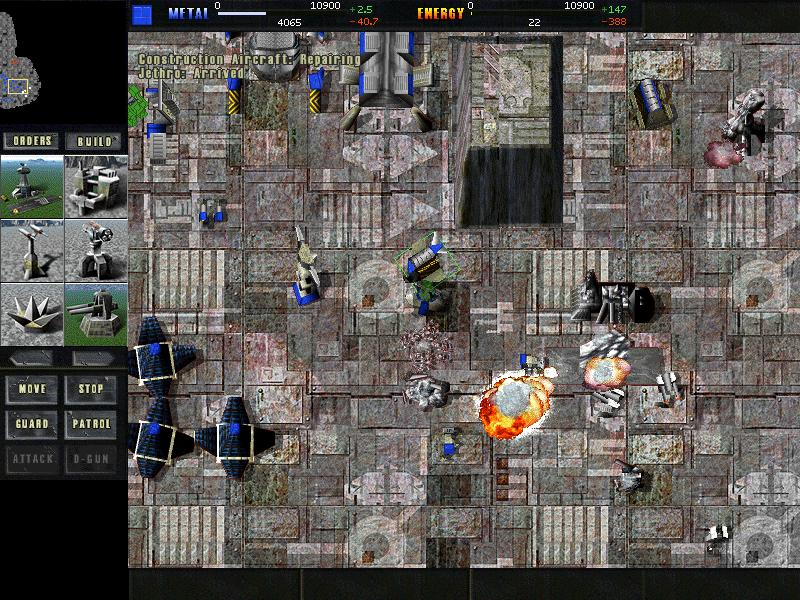
\includegraphics[width=6cm]{res/ta/ta}
	\caption{Total Annihilation screen showing several unit types and some wrecks.}
	\label{fig:ta}
\end{marginfigure}

A game hugely influential in the realm of real-time strategy is \emph{Total Annihilation} (TA), released by by Cavedog Entertainment in 1997. The reception to TA was extremely positive, and the game is still actively played to this day. TA was notable for an advanced resource system that required careful balancing, and 

% Games
% v Gratuitous Space Battles
% x Sins of a Solar Empire
% x Faster Than Light
% v Total Annihilation
% x Mech Commander 2

% likes:
%    - resources allocation to different systems
%    - micro management
%    - upgrading ships by buying weapons
%    - the details of battle effect the overall campaign (repairing damaged parts costs money)
%    - randomly generated campaign (x sectors, then final showdown)
% not likes: 
%    - game play can be stale dependening on ship layout, ie slow guns
%    - resource allocation rather static during battle, changes between battles and start of battle, but not during

Faster Than Light, a turn based strategy game with real time strategy battles, is set in space, with the player taking command of a ship with the objective of getting to the other side of the galaxy.
\begin{marginfigure}
	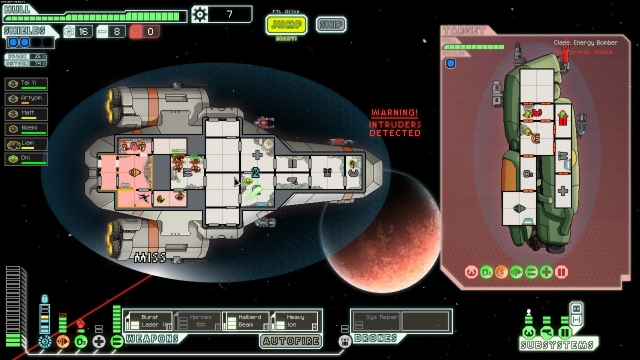
\includegraphics[width=6cm]{res/ftl/ftl}
	\caption{Faster Than Light}
	\label{fig:ftl}
\end{marginfigure}
The ship has an upgrade system that allows the player to upgrade various systems/parts of the ship giving advantages in the next battle, giving the player an incentive to battle, since winning a battle grants currency.
The ship has energy that needs to be allocated to the various systems such as shields, weapons, and life support.
This gives the player a greater control over their ship, whilst allowing them to tweak the capabilities of the ship during battle, ie temporarily dropping life support to boost their weapons.
During battle, the player's responsibilities can vary completely from having to do nothing to having to pause the game every few seconds to calculate the next optimal move. Having a varied level of responsibility adds to the dynamic gameplay, however this game varied too much, ranging from complete boredom to a single battle taking much longer than it should.
A multiplayer mode was missing from the game, causing the gameplay to become predictable, and not replay-able.

% likes
%    - planets would become battlenecks causing the majority of battles to occur their.
%    - different play styles existed where their would be 
% dislikes
%    - game would run way too long
%    - resources would only be used for building, and wouldn't inflence a battle
% dislikes

\begin{marginfigure}
	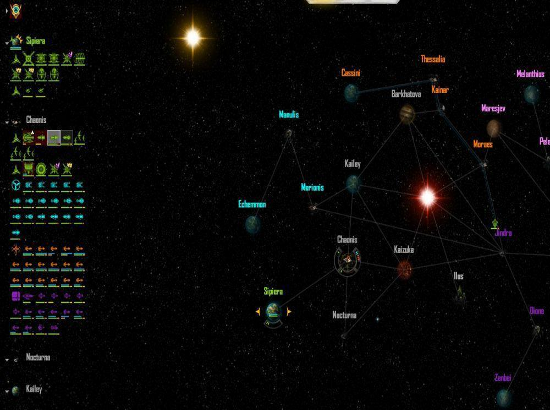
\includegraphics[width=6cm]{res/sins/sins}
	\caption{Sins of a Solar Empire}
	\label{fig:sse}
\end{marginfigure}

Sins a of Solar Empire was a futuristic real time strategy based in space, with the game world modelling a graph of planets, where the player could only move ships between planets that were connected. 
The objective was to wipe out the opposing faction(s) by destroying their ships and capturing their planets.
The gameplay didn't have many twists to the outcome of a battle, resulting in the dominant player continuing to gradually take ground, resulting in very long and boring gameplay.
Due to the layout of the world, certain planets would become bottleneck where the majority of battles occurred. 
A race would ensure to capture these planets that would become the bottlenecks, adding to the player's overall strategy.
The downside of this was that it was apparent who would likely win based on who had captured these bottleneck planets.
The layout of each game was procedurally generated, making each game unique and greatly improving the replay-ability factor for the game.
A resource system existed that had 3 resources: Credits, Metal, and Crystal. 
These resources were only used for the building of fortifications and ships, and would not effect the outcome of the battle directly.


Mech Commander 2 (MC2) is a real-time tactics video game developed by FASA Interactive. The game features simple 3 dimensional graphics and special effects for it's time, but proved to be very popular due to it's unique game style. MC2 allowed the player to deploy a number of mech units (constrained by a maximum weight capacity) to the battlefield. Once on the battlefield the player was vastly outnumbered by enemy mechs and had to rely on stealth and superior tactics to complete a number of objectives. Higher priority objectives were more heavily defended, so the play had to invest more time devising strategies, but received a higher payoff for the mission when they completed the higher priority objectives. What made MC2 particularly interesting was the deployment phase, in which the player had the opportunity to customise mechs with weapons, armour, and system upgrades (e.g. sensors and jump-jets). Mech customisation allowed the player to have full control over their strategies by outfitting mechs to meet their requirements on the battlefield (e.g. Designing a lightweight mech with jump-jets to bait heavier guarding mechs into an ambush).

\begin{marginfigure}
	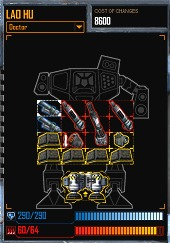
\includegraphics{res/mc2/laohu_lab_half}
	\caption{Mech Commander 2 customise mech screen}
\end{marginfigure}

Gratuitous Space Battles (GSB) could be described as a tower defence game, where the player fully customises a fleet of ships prior to a skirmish but then has no influence over the battle once it begins. Unlike a tower defence game, the objective is simply to eliminate the enemy fleet. GSB provided a very elaborate ship customisation screen, where each component added would affect a large number of the ship's properties (mass, heat capacity, crew required etc.). Although low level unit customisation has proved very popular, GSB took a great risk in scaling the customisation up so much and removing the ability to influence the battle. Overcomplicating the ship building interface led to information overload for new players, making it difficult to understand how many small changes compound and affect the overall design. The lack of control over ships meant boring, drawn out battle scenes. Perhaps one lesson to take from GSB is to keep and customisation interfaces simple, and give players free reign of control as much as possible.


\section{Methodology}

After a considerable number of different ideas were examined and roughly prototyped, a game concept was settled upon. The chosen genre is real time strategy between spaceships, with the emphasis on fast battles that last no longer than half an hour. Differing levels of control are envisaged, where the single flagship might require a high level of detailed control, other ships are given more general orders that an AI then interprets and acts upon.

It is felt that this is a game concept that could compete in the current market and has the potential to be very enjoyable. 
The main part of the project will be development of this game, culminating in user testing, and a full and detailed write up. However it is essential to the aims of the project that the nature of using a functional language is properly captured in this final report. To this end it is planned that during development each programmer will keep a `diary' of code wins/challenges. Any observations about the method need to be captured immediately as they happen, otherwise they won't be remembered with enough clarity at the end to form truly useful insights.

It is hoped that there will be enough material gathered during the development that it can be combined in the final report into a kind of guide to game programming in Haskell. This could form the basis for a much larger piece of work to guide functional development of games or similar applications. Also there will be identified a wish list for future libraries and features available to Haskell programmers.

A significant amount of research has gone into these decisions, which is partly presented later in this document. The final report will give a much more detailed examination of these issues.

\section{Legal, Ethical, and Social Issues}
\label{section:professional_issues}

% legal
One potential legal issue faced by this project is the use of third party software.
It must be ensured that any third party libraries included in the code are licensed
appropriately. This means only using software with a permissive license (e.g. Apache, BSD, or MIT licenses) and no proprietary software.

Game publishers such as Electronic Arts, and Lion Head, consider their games as intelliectual property and copyright their games.
It is infeasible to check that all previous games published do not bear great similarities which could result in a court case.

% ethical
Games can be highly addictive, resulting in their players investing many hours into the game.
If the game is pay-to-play, this can also result in large sums of money invested into the game.
The game being developed uses a fixed length campaign of 5 battles, resulting in convenient game play periods for the user to quit the game.  

% social issues
The game is based in a fictional world, with a non-realistic graphical representation of this world. Current issues with games, such as racism, and violence are not an issue with this game.

The game will only support the english language.
This prevents users from using the game who cannot read english.




\section{Working Title}

Every game needs a working title. \emph{Serenity}, has been chosen as the working title for the game to be produced as part of the project, and the project as a whole has been codenamed \emph{Project Serenity}. As the game becomes more fully developed a more appropriate title may be substituted.
